\chapter{Large Sphere Experiment} %new name?
\label{chap:LargeSphere}

\textit{The work presented here has been presented previously as an oral presentation at AIC 2013 \citep[p. 623]{macdonald_chromatic_2013} \textbf{prior to the author's involvement}, and as an oral presentation at ICVS 2017 \citep[p. 35/58]{jan_kremers_24th_2017} by the author.}

\section{Summary}

The goal of this experimental work was to examine the effect of different wavelengths of light upon chromatic adaptation. Our hypothesis was that \gls{ipRGC} stimulation may need to be considered in order to fully model the induced adaptation, with the null hypothesis being that chromatic adaptation can be fully accounted for by cone and rod mechanisms.

Within a Ganzfeld viewing environment, illuminated by one of 16 different wavelengths of near-monochromatic light, observers performed an achromatic setting task, controlling the chromaticity of a display visible in the central field through a 4$^{\circ}$ circular aperture with two handheld sliders.

Code and data??????? %%%%%

Results:

This project was designed before the author arrived at \gls{UCL}, and data from two participants had already been collected. Data collection required at least 16 hours commitment from observers, and so the only observers up to that point had been LM (one of the authors academic supervisors), who initiated the experiment, and TR who \dots %%%
The original goal for my involvement in this project was that I should be a third observer, and assist in the data analysis. However, following the collection and initial data analysis of my own data, it became clear that there had been a technical fault during this run of data collection, and my data was deemed corrupted. This data is discussed further in Appendix X. %%%%%%%%
Thus, my only contribution to this work is an extension to the data analysis started by LM, upon which I shall focus on in this chapter.

\section{Methodology}

\subsection{Hardware}

A hollow fibreglass sphere of approximately 750mm diameter was prepared with three holes; the first for an observer's face, the second (above) for an illuminant to illuminate the Ganzfed, and the third (opposite the first) through which a small portion of an LCD screen could be seen. The interior of the sphere was painted with RAL 7040 dulux vinyl matt, of approximately 38\% reflectance. Illumination was provided by a Kodak slide projector, filtered through one of 16 near-monochromatic filters, ranging in 20nm intervals from 400-700nm inclusive.

\begin{figure}[htbp]
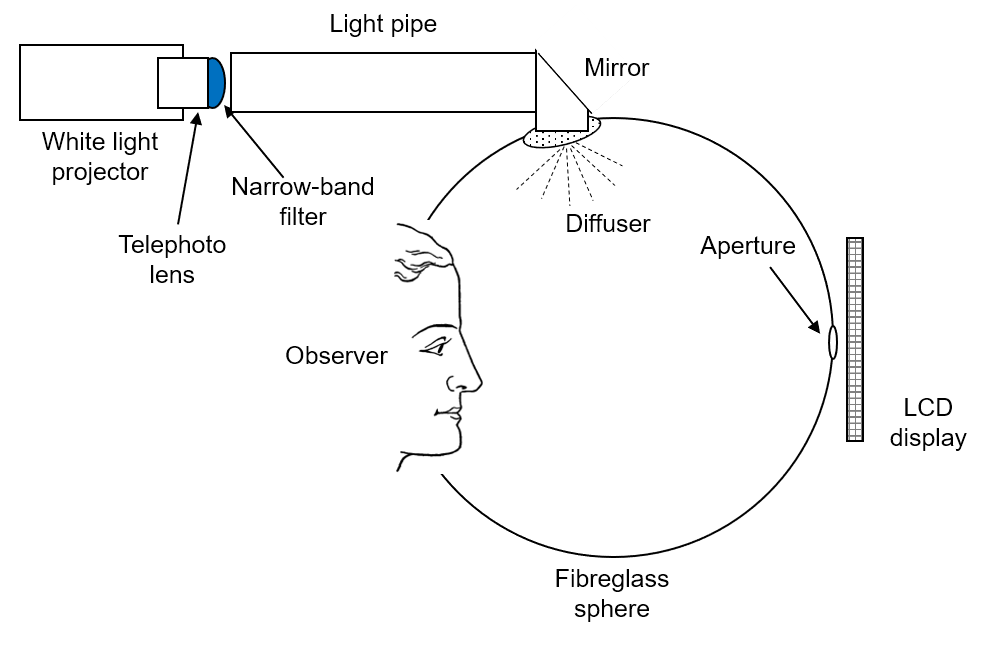
\includegraphics[max width=\textwidth]{figs/LargeSphere/sketch.png}
\caption{The hardware design. Illustration courtesy of Lindsay MacDonald.}
\label{fig:sketch}
\end{figure}

\begin{figure}[htbp]
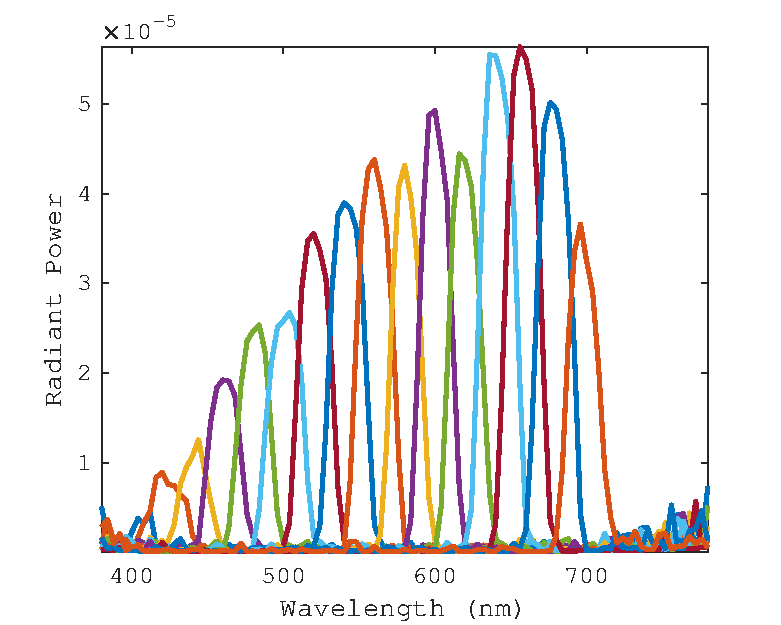
\includegraphics[max width=\textwidth]{figs/LargeSphere/LSillum.pdf}
\caption{The illuminants within the sphere, created by filtering light from a slide projector, measured as reflecting from a point just to the right of the aperture through which an observer would view the screen. Measurements made by Lindsay MacDonald.} %%%%%%?????
\label{fig:LSillum}
\end{figure}

\subsection{Observer task}

The observer sat on one side of the sphere with their face inside the sphere, such that nothing outside of the sphere was visible. On view on the opposite side of the sphere was a circular 4$^{\circ}$ aperture onto an LCD screen, upon which a random colour drawn from ??????%
was visible. It was the observer's task to use two handheld sliders, which controlled the chromaticity of the screen, to make the appearance of the screen achromatic. Once they were happy with the achromacy of the patch, they were to hit a button at which a new random colour would be presented. The first displayed colour was displayed at L* of 85, with subsequent colours descending by 5 L* until 15 L*. This scale was repeated 10 times per session. Per session observers made 10 selections at 16 lightness levels (160 total). Observers performed 16 sessions (2560 selections total). See Figure \ref{fig:ExperimentalPro}.

\begin{figure}[htbp]
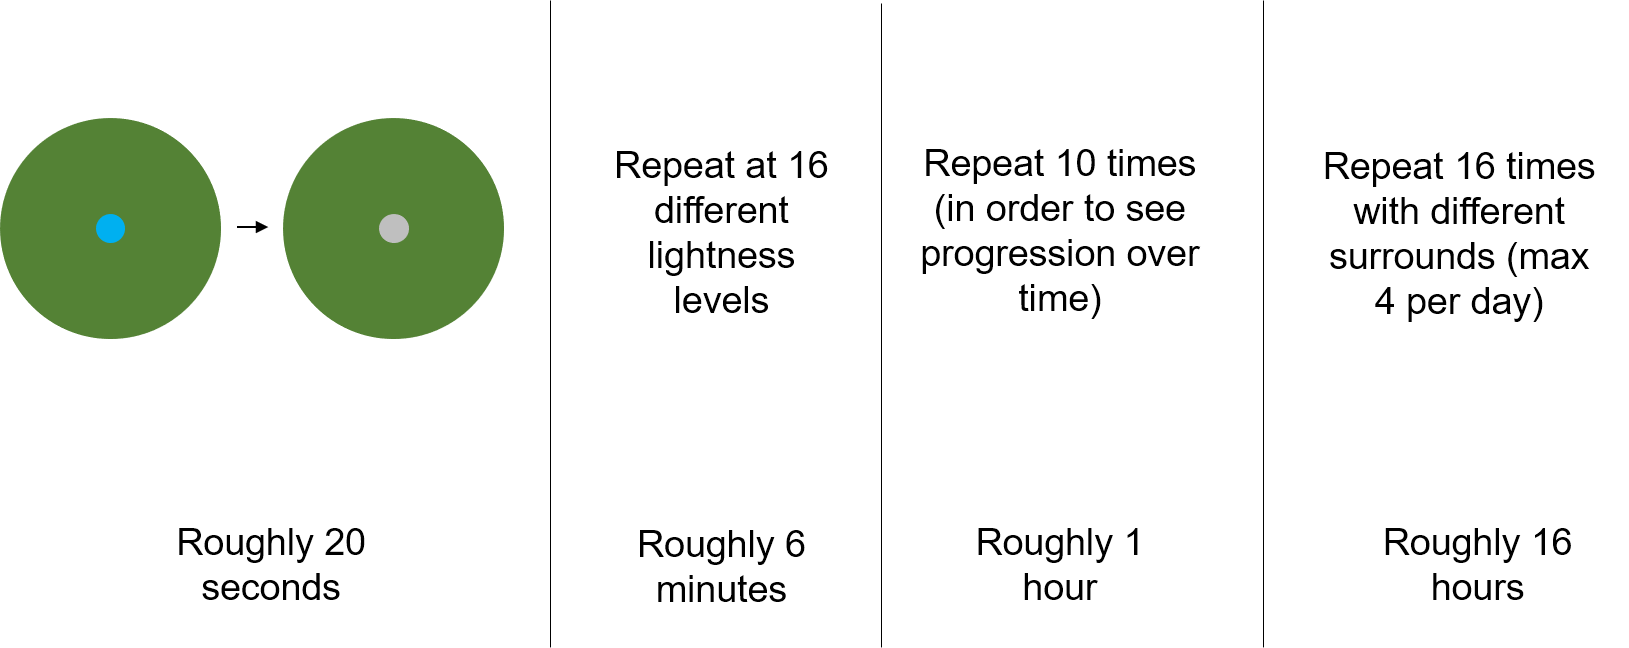
\includegraphics[max width=\textwidth]{figs/LargeSphere/ExperimentalPro.png}
\caption{The experimental protocol.}
\label{fig:ExperimentalPro}
\end{figure}

\subsection{Data Collection}

Data was collected for two observers \dots

\subsection{Data Processing}

Two distinct approaches were taken to data processing. The first attempted to process the data in a chromatic space, with the reasoning that under the null condition chromatic selections should simply correspond to the chromaticity of the surround illuminants. If it were shown that this relationship was not as expected, in a manner which might suggest involvement by other mechanisms (meaning rods or \glspl{ipRGC}), then this could be considered as evidence against the null hypothesis.

The second approach took advantage of the fact that measurements were taken at samples across the wavelength spectrum. Here the logic was that if the null condition were true, we should be able to fit a model to observer responses which only used cone-based inputs, and we could carefully consider the (presumed) benefit of including rods and \glspl{ipRGC} in the model. If either rod input of \gls{ipRGC} input were found to dramatically improve the model then this could be considered as evidence against the null hypothesis.

\section{Results}

\subsection{Chromaticity-based analysis}

\hl{As presented at ICVS.}

\subsection{Spectrum-based analysis}

The first stage of this analysis was to generate simulated data which represented the situation whereby there was only simple Von Kries adaptation, with no bounds on selections considered. This was accomplished by multiplying the individual \glspl{SPD} (Figure \ref{fig:LSillum} by the CIE 2006 10$^{\circ}$ observer fundamentals (not in the manner in which this is usually done, resulting in tristimulus values, but rather retaining a spectral nature to the data).

\begin{figure}[htbp]
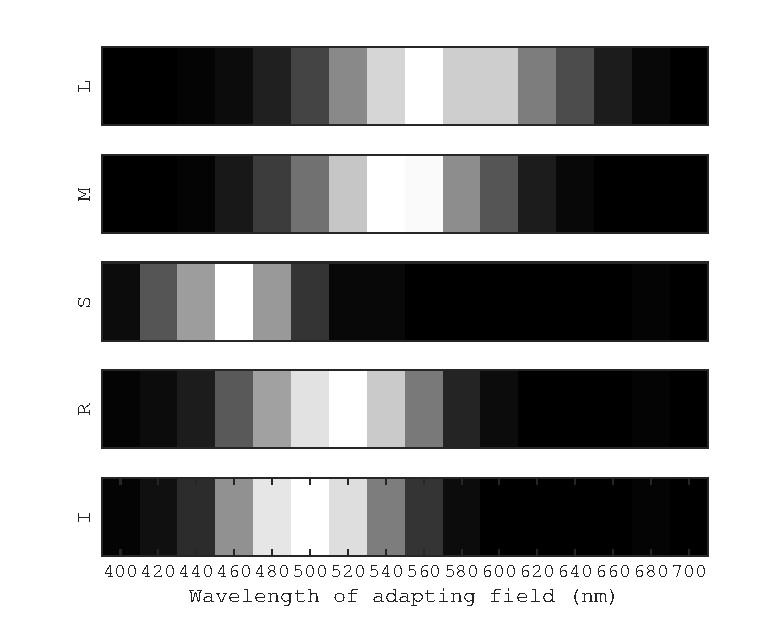
\includegraphics[max width=\textwidth]{figs/LargeSphere/LSsimdata.pdf}
\caption{Simulated data for a basic Von Kries observer. In this figure white represents a high response. For example, with 560nm peripheral stimulation we would expect an observer to pick a colour with high L-cone activation as achromatic, assuming that the sensitivity of L-cones had been suppressed and thus higher activation was required to reach a neutral point.}
\label{fig:LSsimdata}
\end{figure}

A comparison was then made between this data and a set of real data (Obs = TR, averaged over time (entire run, no exclusions), averaged over L* = 35:60\footnote{Values outside of this range exhibited gamut boundary issues.}). This real data had been transformed from the recorded blablabla %!!!!!! 
values into L,M,S values analogous to the simulated data. It can be seen however that there is a considerable difference between the simulated data and the real data (Figure \ref{fig:simVreal}. S-cone data shows the closest match, with the predicted peak at 480 being mirrored in the real data. This peak appears to bleed into the M-cone data, and the simulated data for L and M-cone data shows very little correspondence to the collected data. Correlations are:

\begin{figure}[htbp]
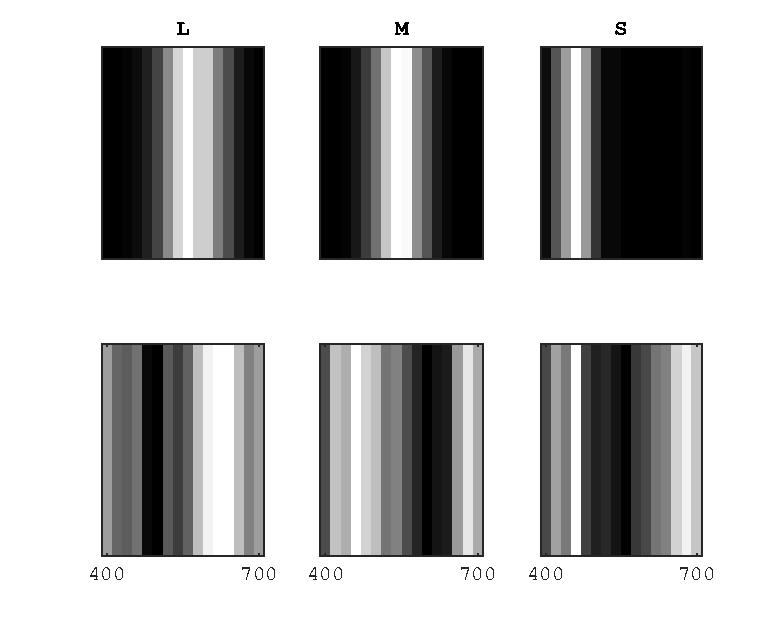
\includegraphics[max width=\textwidth]{figs/LargeSphere/simVreal.pdf}
\caption{A comparison of simulated data (top row) and real data (bottom row).}
\label{fig:simVreal}
\end{figure}

In order to understand the way in which adaptation may be crossing between channels, or the way in which we may have not properly isolated our channels (it is unclear exactly how much freedom an observer truly has to move around the response space) a brute-force method was used to find combinations of the above simulated data which would best fit the real data.

X random sets of weightings (X total) between X and X were generated. These weightings were applied to the simulated responses and the responses were additively combined. The correlation between this new data and the real data was calculated. The top performing randomly generated datasets were selected and are presented in X. These correlated with the data at X,Y,Z. These are much improved over X.

\begin{figure}[htbp]
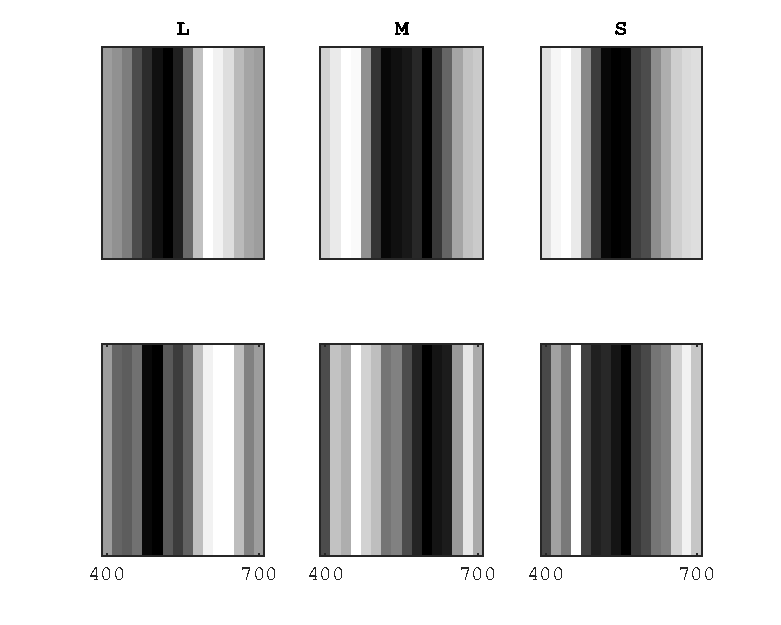
\includegraphics[max width=\textwidth]{figs/LargeSphere/maxsimVreal.pdf}
\caption{A comparison of simulated data following a brute force recombination (top row) whereby channels were freely mixed to best correlate with real data, and real data (bottom row).}
\label{fig:maxs (asimVreal}
\end{figure}

The top X\% of generated data are presented in terms of their components in figure X.

Adding in rods gave maximal correlations of: 
Adding in melanopsin gave maximal correlations of:
Adding both gave:

This is a minimal improvement. Therefore, I do not reject the null hypothesis in this case.

Further investigations might add time dependency

Try the other datasets we have //
\dots possibly with more precise observer models for each.

I’d also like to try having a different observer for central and peripheral.

Consider different time points.	



%Simplifications were made to consider only an average L* value (between and one timepoint 

\section{Discussion}
\section{Conclusion}